\documentclass[ignorenonframetext,xcolor=x11names]{beamer}

\input{../common.preamble.beamer.tex}

\title{Business 4720 - Class 21}

\subtitle{Reinforcement Learning -- Tabular Methods}

\begin{document}

\begin{frame}{}
  \titlepage
  \footnotesize
  \input{../license.tex}
\end{frame}

\section{Introduction}

\begin{frame}{This Class}

\begin{block}{What You Will Learn:}
\begin{itemize}
  \item Reinforcement Learning
  \begin{itemize}
     \item Multi-Armed Bandits
     \item Value Functions
     \item Monte-Carlo (MC) Methods
     \item Temporal-Difference (TD) Methods
  \end{itemize}
\end{itemize}
\end{block}
\end{frame}

\begin{frame}{Based On}
\begin{block}{}
Richard S. Sutton and Andrew G. Barto (2018) \emph{Reinforcement Learning -- An Introduction}. 2nd edition, The MIT Press, Cambridge, MA. (SB) \\
\vspace{0.5\baselineskip}
\url{http://incompleteideas.net/book/the-book.html} \\
\vspace{0.5\baselineskip}
Chapters 2--7 \\
\vspace{0.5\baselineskip}
(CC BY-NC-ND License)
\end{block}
\end{frame}

\begin{frame}{Resources}
Implementations are available on the following GitHub repo:

\url{https://github.com/jevermann/busi4720-rl} \\


The project can be cloned from this URL:

\url{https://github.com/jevermann/busi4720-rl.git}
\end{frame}

\begin{frame}{Reinforcement Learning}
\centering  \textbf{Online Learning by Acting in an Environment}
\vspace{\baselineskip}  
\begin{block}{Ideas}
\begin{itemize}
   \item Maximize return
   \item Immediate and delayed/subsequent rewards
   \item Discover which actions to take by trying them
   \item Tradeoff between exploration and exploitation
   \item Uncertain/random/stochastic environment
\end{itemize}
\end{block} 
\vspace{\baselineskip} \centering
\emph{Problem cannot be tackled by optimization (e.g. dynamic programming), because of incomplete knowledge of environment.}
\end{frame}

\begin{frame}{Reinforcement Learning}
\begin{block}{Core Concepts}
\begin{itemize}
    \item \textbf{Policy} $\pi$ (probability of taking action $a$ in state $s$)
    \item \textbf{Reward} $R$ (received from the environment after each action)
    \item \textbf{Return} $G$ (possibly discounted sum of future rewards)
    \item \textbf{State value function} $v$ (expected return for each state)
    \item \textbf{Action value function} $q$ \\ (expected return for each state and action)
    \item \textbf{Model} $p$ (behaviour of the environment, optional)
\end{itemize}
\end{block}
\end{frame}

\begin{frame}{Introductory Example -- Tic-Tac-Toe \small(Naughts and Crosses)}
\begin{columns}
\begin{column}{0.25\textwidth}
\includegraphics[width=\textwidth]{Tic_tac_toe.png} \\
\vspace{\baselineskip}
\scriptsize \url{https://commons.wikimedia.org/wiki/File:Tic_tac_toe.svg}
\end{column}
\begin{column}{0.75\textwidth}
\begin{itemize}
  \item Value is probability of winning from state
  \item Value of any state with X-X-X is 1.0
  \item Value of any state with O-O-O or full board is 0.0
  \item Initial values are 0.5
\end{itemize}
\end{column}
\end{columns}
\end{frame}

\begin{frame}{Introductory Example -- Tic-Tac-Toe \small [cont'd]}
\begin{columns}
\begin{column}{0.5\textwidth}
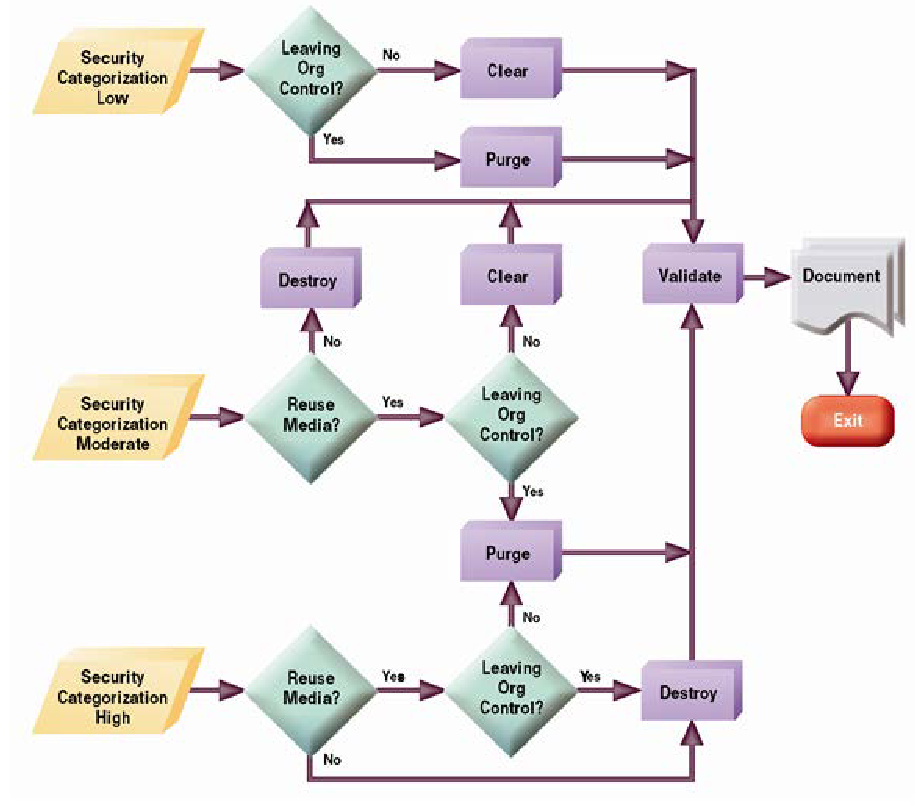
\includegraphics[width=1.1\textwidth]{screen1.png} \\
\centering
\scriptsize Source: SB Figure 1.1
\end{column}
\begin{column}{0.5\textwidth}
\begin{itemize}
  \item Normally, move \emph{greedily} to highest-valued next state
  \item Sometimes, make random \emph{exploratory} move
  \item After each greedy move, update state value towards value of later state with \emph{step size} $\alpha$
  \item \emph{Temporal-difference} learning $V(S_{t+1}) - V(S_t)$
  \item Take advantage of information \emph{during} episode/game.
\end{itemize}
\end{column}
\end{columns}
  \begin{align*}
  V(S_t) \leftarrow V(S_t) + \alpha \left[ V(S_{t+1}) - V(S_t)\right] 
  \end{align*}
\end{frame}

\begin{frame}{Example Applications in Business and Management}
\begin{itemize}
  \item \textbf{Marketing}: Learn which online ads to show to which site visitor
  \item \textbf{HR}: Learn which employee to assign to which task
  \item \textbf{Operations}: Learn which work item to assign to which machine
  \item \textbf{Logistics}: Learn which item to route on which truck or flight
  \item \ldots
\end{itemize}
\end{frame}

\begin{frame}{K-armed Bandits}
\begin{columns}
\begin{column}{.2\textwidth}
\includegraphics[width=1.2\textwidth]{one-armed_bandit.jpg}\\
\tiny \url{https://commons.wikimedia.org/wiki/File:Antique_one-armed_bandit,_Ventnor,_Isle_of_Wight,_UK.jpg}
\end{column}
\begin{column}{.8\textwidth}
\small
\begin{itemize} 
   \item Stateless environment
   \item $k$ possible actions $A_t$ at time $t$ with stochastic reward $R_t$
   \item Estimate \emph{action value} as:
   \begin{align*}
   Q_t(a) = \frac{\sum_{i=1}^{t-1} R_i \times \mathbbm{1}_a}{\sum_{i=1}^{t-1} \mathbbm{1}_a} \qquad \text{(average reward)}
   \end{align*} \vspace{-.5\baselineskip}
   \item $\epsilon$\emph{-greedy policy}: With probability $\epsilon$ take random action, with probability $1-\epsilon$ take optimal action
   \begin{align*}
   A_t = \operatorname*{arg max}_a Q_t(a)
   \end{align*} \vspace{-\baselineskip}
   \item Incremental implementation
   \begin{align*}
   Q_{t+1}(a) = Q_t(a) + \frac{1}{t}\left[R_t(a) - Q_t(a)\right]
   \end{align*}
\end{itemize}
\end{column}
\end{columns}
\end{frame}

\begin{frame}{General Update Rule for Estimates}
\begin{align*}
NewEstimate \leftarrow OldEstimate + StepSize \left[ Target - OldEstimate \right]
\end{align*}

\vspace{\baselineskip}
$\left[ Target - OldEstimate \right]$ is the \emph{error} in the estimate
\end{frame}

\begin{frame}{K-armed Bandits -- Example}
\begin{block}{A simple bandit algorithm}
Initialize, for $a=1$ to $k$:
\begin{align*}
&\quad Q(a) \leftarrow 0 \\
&\quad N(a) \leftarrow 0
\end{align*}
Loop forever:
\begin{align*}
&\quad A \leftarrow \begin{cases} \operatorname*{arg max}_a Q(a) &\qquad \text{with probability}\, 1-\epsilon \\
\text{a random action} &\qquad \text{with probability}
\, \epsilon
\end{cases} \\
&\quad R \leftarrow \operatorname{bandit}(A) \\
&\quad N(A) \leftarrow N(A) + 1 \\
&\quad Q(A) \leftarrow Q(A) + \frac{1}{N(A)} \left[ R - Q(A) \right]
\end{align*}
\end{block}
\end{frame}

\begin{frame}[fragile]{K-armed Bandits -- Python}
Environment:
\begin{pythoncode}
class k_bandit_env:
    def __init__(self, k):
        self.k = k
        self.mean_rewards = []

        for i in range(self.k):
            self.mean_rewards \
                .append(random.normalvariate(0, 1))

    def step(self, action):
        mean = self.mean_rewards[action]
        reward = random.normalvariate(mean, 1)
        return reward
\end{pythoncode}
\end{frame}

\begin{frame}[fragile]{K-armed Bandits -- Python}
Agent:
\begin{pythoncode}
class k_bandit_agent:
    def __init__(self, k, epsilon, initial_value):
        self.k = k
        self.epsilon = epsilon
        self.env = k_bandit_env(k)

        self.Q = [initial_value] * self.k
        self.N = [.0] * self.k

    def determine_action(self):
        if random.uniform(0,1) < self.epsilon:
            # explore
            action = random.randint(0, self.k-1)
        else:
            # exploit
            action = self.Q.index(max(self.Q))
        return action
\end{pythoncode}
\end{frame}

\begin{frame}[fragile]{K-armed Bandits -- Python}
Agent (continued):
\begin{pythoncode}
    def train(self, steps):
        rewards = []
        for step in range(steps):
            action = self.determine_action()
            reward = self.env.step(action)
            self.N[action] += 1
            self.Q[action] = \
               (reward-self.Q[action])/self.N[action]
            rewards.append(reward)
        return rewards
\end{pythoncode}
\begin{center}
Complete implementation at \\
\vspace{\baselineskip}
\url{https://evermann.ca/busi4720/bandits.py}
\end{center}
\end{frame}

\begin{frame}{K-armed Bandits -- Policy Comparison}
Values for $\epsilon$ and the initial $Q$ value affect learning behaviour:

\includegraphics[width=\textwidth]{bandits.pdf}
\end{frame}

\begin{frame}{Markov Decision Processes}
\begin{center}
\includegraphics[width=0.75\textwidth]{screen3.png} \\

\scriptsize Source: SB Figure 3.1 \normalsize
\end{center}
\begin{itemize}
   \item \textbf{Trajectory}: 
\begin{align*}S_0, A_0, R_1, S_1, A_1, R_2, \ldots
\end{align*}
   \item \textbf{Dynamics}: 
\begin{align*}p(s', r | s, a) = Pr\{S_t = s', R_t =r | S_{t-1} = s, A_{t-1} = a \}
\end{align*}
\end{itemize}
\end{frame}

%\begin{frame}{Markov Decision Processes \small [cont'd]}
%\begin{itemize}
   %\item \textbf{State-transition probabilities}: 
%\begin{align*}
%p(s' | s, a) = Pr\{S_t = s' | S_{t-1} =s , A_{t-1} = a \} = \sum_{r \in \mathcal{R}} p(s', r|s, a)
%\end{align*}
   %\item \textbf{Expected reward}: 
%\begin{align*}
%r(s, a) = \mathbbm{E}[R_t | S_{t-1} =s , A_{t-1}=a] = \sum_{r \in \mathcal{R}} r \sum_{s' \in \mathcal{S}} p(s', r|s, a)
%\end{align*}
   %\item \textbf{Discounted return}:
%\begin{align*}
%G_t &= R_{t+1} + \gamma R_{t+2} + \gamma^2 R_{t+3} + \cdots = \sum_{k=0}^{\infty} \gamma^k R_{t+k+1} \\
    %&= R_{t+1} + \gamma G_{t+1}
%\end{align*}
%\end{itemize}
%\end{frame}

\begin{frame}{Markov Decision Processes \small [cont'd]}
\begin{itemize}
   \item \textbf{Discounted future return}:
\begin{align*}
G_t &= R_{t+1} + \gamma R_{t+2} + \gamma^2 R_{t+3} + \cdots = \sum_{k=0}^{\infty} \gamma^k R_{t+k+1} \\
    &= R_{t+1} + \gamma G_{t+1}
\end{align*}
  \item \textbf{State value function} of state $s$ under a policy $\pi$:
\begin{align*}
v_\pi(s) = \mathbbm{E}_\pi [ G_t | S_t = s] = \mathbbm{E}_\pi \left[ \sum_{k=0}^\infty \gamma^k R_{t + k + 1} | S_t = s \right]
\end{align*}
  \item \textbf{Action value function} for policy $\pi$:
\begin{align*}
q_\pi(s, a) &= \mathbbm{E}_\pi [ G_t | S_t = s, A_t = a] \\
&= \mathbbm{E}_\pi \left[ \sum_{k=0}^\infty \gamma^k R_{t + k + 1} | S_t = s, A_t = a \right]
\end{align*}
\end{itemize}
\end{frame}

\begin{frame}{Bellman Equation}
The value function $v$ for policy $\pi$ is the unique solution to the \textbf{Bellman equation}:
\begin{align*}
v_\pi(s) &= \mathbbm{E}_\pi [ G_t | S_t = s] \\
&= \mathbbm{E}_\pi [R_{t+1} + \gamma G_{t+1} | S_t = s] \\
&= \sum_a \pi(a | s) \sum_{s'} \sum_r p(s', r | s, a) \left[ r + \gamma \mathbbm{E}_\pi [ G_{t+1} | S_{t+1} = s'] \right] \\
&= \sum_a \pi(a | s) \sum_{s', r} p(s', r | s, a) \left[r + \gamma v_\pi(s') \right] \quad \text{for all} \, s \in \mathcal{S}
\end{align*}
\centering
\footnotesize{(Recall: Expected value is sum weighted by probabilities)}
\end{frame}

\begin{frame}{MDP -- Gridworld State Value Function}
\begin{itemize}
   \item Actions: Up, Down, Left, Right
   \item Falling off the world results in reward of $-1$ 
   \item Other actions result in reward of $0$, except for $A$ to $A'$ and $B$ to $B'$ as indicated
   \item Policy $\pi$ is to take each action with equal probability
   \item Discount rate $\gamma = 0.9$
\end{itemize}
\begin{center}
\includegraphics[width=\textwidth]{screen4.png} \\

\scriptsize Source: SB Figure 3.2 \normalsize
\end{center}
\end{frame}

\begin{frame}{MDP -- Optimal Policies}
Maximizing the state value function $v$ or action value function $q$ is finding an optimal policy $\pi$:
\begin{align*}
v_*(s) &= \operatorname*{max}_\pi v_\pi(s) \\
q_*(s, a) &= \operatorname*{max}_\pi q_\pi(s, a)
\end{align*}
%\intertext{$q_*$ can be expressed in terms of $v_*$:}
%q_*(s, a) &= \mathbb{E} [ R_{t+1} + \gamma v_* (S_{t+1}) | S_t =s , A_t =a ]
%\end{align*}
Intuitively, the value of a state under an optimal policy $\pi_*$ is equal to the expected return for the the best action from that state:
\begin{align*}
v_*(s) &= \max_{a \in \mathcal{A}(s)} q_{\pi_*} (s, a) \\
\end{align*}
\end{frame}


\begin{frame}{MDP -- Bellman Optimality}
\begin{align*}
v_*(s) &= \max_{a \in \mathcal{A}(s)} q_{\pi_*} (s, a) \\
&= \max_a \mathbb{E}_{\pi_*} [ G_t | S_t =s , A_t = a ] \\
&= \max_a \mathbb{E}_{\pi_*} [R_{t+1} + \gamma G_{t+1} | S_t =s, A_t =a ] \\
&= \max_a \mathbb{E} [ R_{t+1} + \gamma v_* (S_{t+1}) | S_t =s , A_t =a ] \\
&= \max_a \sum_{s', r} p(s', r | s, a) [ r + \gamma v_* (s')]
\end{align*}
Similarly for action value under an optimal policy:
\begin{align*}
q_*(s, a) &= \mathbb{E} \left[ R_{t+1} + \gamma \max_{a'} q_*(S_{t+1}, a') | S_t = s, A_t =a \right] \\
&= \sum_{s', r} p(s', r | s, a) [ r + \gamma \max_{a'} q_* (s', a') ]
\end{align*}
\end{frame}

\begin{frame}{Dynamic Programming}
\begin{block}{Intuition:}
  \begin{enumerate}
     \item Start from random value function and policy
     \item Compute updated value function (iteratively)
     \item Adjust policy based on updated value function
     \item Repeat from (2) until convergence
  \end{enumerate}
\end{block}
\end{frame}

\begin{frame}{Dynamic Programming}
\begin{block}{Iterative Policy Evaluation}
\begin{align*}
&\text{Loop:} \\
&\quad \Delta \leftarrow 0 \\
&\quad \text{Loop for each}\, s \in \mathcal{S}: \\
&\quad \quad v \leftarrow V(s) \\
&\quad \quad V(s) \leftarrow \sum\nolimits_a \pi(a|s) \sum\nolimits_{s', r} p(s', r|s, a)[r + \gamma V(s')] \\
&\quad \quad \Delta \leftarrow \max (\Delta, |v - V(s)|) \\
&\text{until}\, \Delta < \theta
\end{align*}
\end{block}
\end{frame}

\begin{frame}[fragile]{Iterative Policy Evaluation in Python}
\begin{pythoncode}
# Initialize value function V
V = dict()
for state in States:
    V[state] = 0
# Initialize policy pi
pi = dict()
for state in States:
    pi[state] = 0

def evaluate_policy():
    while True:
        Delta = 0
        for s in States:
            v = V[s]
            V[s] = exp_reward(s, pi[s])
            Delta = max(Delta, abs(v - V[s]))
        print(Delta)
        if Delta < theta:
            break
\end{pythoncode}
\end{frame}

\begin{frame}{Dynamic Programming}
\begin{block}{Iterative Policy Improvement}
\begin{align*}
&\text{Loop:} \\
&\quad stable \leftarrow true \\
&\quad \text{For each}\, s \in \mathcal{S}: \\
&\quad \quad old\_action \leftarrow \pi(s) \\
&\quad \quad \pi (s) \leftarrow \operatorname*{argmax}\nolimits_a \sum\nolimits_{s', r} p(s', r|s, a) [r + \gamma V(s')] \\
&\quad \quad \text{If}\, old\_action \neq \pi(s) \, \text{then} \, stable \leftarrow false \\
&\quad \text{If}\, stable \; \text{then} \\
&\quad \quad \text{return}\, V \approx v_*\, \text{and} \, \pi \approx \pi_* \\
&\quad \text{else} \\
&\quad \quad \text{go to policy evaluation}
\end{align*}
\end{block}
\end{frame}

\begin{frame}[fragile]{Iterative Policy Improvement in Python}
\begin{pythoncode}
def improve_policy():
    stable = True
    for s in States:
        old_action = pi[s]
        max_r = -math.inf
        max_a = None
        for action in Actions:
            r = exp_reward(s, action)
            if r > max_r:
                max_r = r
                max_a = action
        pi[s] = max_a
        if old_action != pi[s]:
            stable = False
    return stable
\end{pythoncode}
\end{frame}

\begin{frame}[fragile]{Iterative Policy Improvement in Python}
\begin{pythoncode}
stable = False
while not stable:
    evaluate_policy()
    stable = improve_policy()

print("Optimal Policy:")
print(pi)
\end{pythoncode}
\begin{center}
Complete implementation at \\
\vspace{\baselineskip}
\url{https://evermann.ca/busi4720/jacks.py}
\end{center}
\end{frame}

\begin{frame}[fragile]{Example -- Jack's Car Rental}
\begin{itemize}
   \item Jack rents cars at 2 locations with capacity of 20 cars
   \item Daily rental requests and returns are Poisson distributed
   \item Move a maximum of 5 cars between locations overnight
   \item $-2$ reward for each move, $+10$ reward for each satisfied rental request
   \item How many vehicles to move each night?
\end{itemize}
\begin{pythoncode}
States = []
for cars1 in range(21):
    for cars2 in range(21):
        States.append((cars1, cars2))
        
Actions = range(-5, 5+1)
\end{pythoncode}
\end{frame}

\begin{frame}{Example -- Policies and Final Value Function}
Policies after each improvement, starting with random initial policy. Final state value function at bottom right. \\

\vspace{.5\baselineskip}
\begin{tabular}{ccc}
\includegraphics[width=0.3\textwidth]{rl_into/jacks_init_random/jacks_pi_iteration_0.png} &
\includegraphics[width=0.3\textwidth]{rl_into/jacks_init_random/jacks_pi_iteration_1.png} &
\includegraphics[width=0.3\textwidth]{rl_into/jacks_init_random/jacks_pi_iteration_2.png} \\
\includegraphics[width=0.3\textwidth]{rl_into/jacks_init_random/jacks_pi_iteration_3.png} &
\includegraphics[width=0.3\textwidth]{rl_into/jacks_init_random/jacks_pi_iteration_4.png} &
\includegraphics[width=0.3\textwidth]{rl_into/jacks_init_random/jacks_V_iteration_4.png}
\end{tabular}
\end{frame}


\begin{frame}{Monte Carlo Methods}
\begin{itemize}
   \item In practice, dynamics of the environment are not known, i.e. $p(s', r | s, a)$ is unknown; there is \emph{no model} of the environment
   \item Learning $V$ and $Q$ from \emph{experience}, ie. sample sequences of states, actions, and rewards. 
   \item Consider \emph{episodic tasks}, with a terminal state and finite returns
   \item Create episodes following policy $\pi$ by interacting with environment
   \item Similar to the bandit problem, which also learned an action value function, but now with states
\end{itemize}
\end{frame}

\begin{frame}{First-visit MC Prediction}
\begin{itemize}
   \item Estimate $V \approx v_{\pi}$
   \item Return assigned to state is that of first visit of state
\end{itemize}

\begin{block}{}
\footnotesize
\begin{align*}
& \text{Input: a policy}\;\pi\;\text{ to be evaluated} \\
& \text{Initialize:} \\
& \quad V(s) \in \mathbbm{R}, \text{arbitrarily, for all}\;s \in \mathcal{S} \\
& \quad Returns(s) \leftarrow \text{an empty list, for all}\; s \in \mathcal{S} \\
& \text{Loop forever (for each episode):}\\
& \quad \text{Generate an episode following}\, \pi: S_0, A_0, R_1, S_1, A_1, R_2, \ldots, S_{T-1}, A_{T-1}, R_{T} \\
& \quad G \leftarrow 0 \\
& \quad \text{Loop for each step of episode,}\; t = T-1, T-2, \ldots, 0: \\
& \quad \quad G \leftarrow \gamma G + R_{t+1} \\
& \quad \quad \text{Unless}\; S_t\; \text{appears in}\; S_0, S_1, \ldots, S_{t-1}: \\
& \quad \quad \quad \text{Append}\; G\; \text{to}\; Returns(S_t) \\
& \quad \quad \quad V(S_t) \leftarrow \operatorname{average}(Returns(S_t))
\end{align*}
\end{block}
\end{frame}

\begin{frame}{MC Control}
\begin{itemize}
   \item State-value function $V$ not useful without model
   \item Estimate action-value function $Q$ and $\pi \approx \pi_*$ directly
   \item To ensure all state-action pairs are visited with a greedy policy, set these as episode starts with some probability (\emph{''exploring starts'', ES})
\end{itemize}
\end{frame}

\begin{frame}{MC Control (ES)}
\begin{block}{}
\footnotesize
\begin{align*}
& \text{Initialize for all}\; s \in \mathcal{S}, a \in \mathcal{A} \\
& \quad \pi(s) \in \mathcal{A}(s) \; \text{(arbitrarily)} \\
& \quad Q(s,a) \in \mathbbm{R}\; \text{(arbitrarily)} \\
& \quad Returns(s, a) \leftarrow \text{empty list} \\
& \text{Loop forever (for each episode):} \\
& \quad \text{Choose}\; S_0 \in \mathcal{S}, A_0 \in \mathcal{A}(S_0)\; \text{randomly} \\
& \quad \text{Generate an episode following}\, \pi: S_0, A_0, R_1, S_1, A_1, R_2, \ldots, S_{T-1}, A_{T-1}, R_{T} \\
& \quad G \leftarrow 0 \\
& \quad \text{Loop for each step of episode,}\; t = T-1, T-2, \ldots, 0: \\
& \quad \quad G \leftarrow \gamma G + R_{t+1} \\
& \quad \quad \text{Unless the pair}\; S_t, A_t \; \text{appears in}\; S_0, A_0, S_1, A_1, \ldots, S_{t-1}, A_{t-1}: \\
& \quad \quad \quad \text{Append}\; G\; \text{to}\; Returns(S_t, A_t) \\
& \quad \quad \quad Q(S_t, A_t) \leftarrow \operatorname{average}(Returns(S_t, A_t)) \\
& \quad \quad \quad \pi(S_t) \leftarrow \operatorname{arg max}_a Q(S_t, a)
\end{align*}
\end{block}
\end{frame}

\begin{frame}{MC (ES) Control Example -- Black Jack}
\begin{itemize}
   \item Card values A, 2, 3, \ldots, 10
   \item Ace can be 1 or 11 (''usable ace'')
   \item Actions: take another card (''hit)'' or do not (''stick'')
   \item Dealer showing initial card, stands on 17 or more
   \item Over 21 is ''bust'' (lost), otherwise closest to 21 wins
\end{itemize}
\end{frame}

\begin{frame}[fragile]{MC (ES) Control Example -- Black Jack}
Define states $\mathcal{S}$ and actions $\mathcal{A}$:
\begin{pythoncode}
gamma = 1.0
# Define states
States = []
for ace in [0,1]:
    for dealer_showing in range(1,11):
        for hand_sum in range(12, 22):
            States.append((ace,dealer_showing,hand_sum))

# Define actions
Actions = (0, 1)
\end{pythoncode}
\end{frame}

\begin{frame}[fragile]{MC (ES) Control Example -- Black Jack}
Initialize policy $\pi$, action-value function $Q$, and returns:
\begin{pythoncode}
# Initialize policy
pi = dict()
for s in States:
    pi[s] = random.randint(0,1)

# Initialize action value function
Q = dict()
for s in States:
    for a in Actions:
        Q[(s, a)] = 0

# Initialize returns
Returns = dict()
for s in States:
    for a in Actions:
        Returns[(s, a)] = []
\end{pythoncode}
\end{frame}


\begin{frame}[fragile]{MC (ES) Control Example -- Black Jack}
Generate an episode using policy $\pi$ from initial state $S_0$ and initial action $A_0$:
\begin{pythoncode}
def generate_episode(pi, s0, a0):
    terminal = False
    s = s0
    a = a0
    states = [s0]
    actions = [a0]
    rewards = [math.nan]
    while terminal is False:
        sprime, r, terminal = step(s, a)
        rewards.append(r)
        if not terminal:
            aprime = pi[sprime]
            states.append(sprime)
            actions.append(aprime)
            s = sprime
            a = aprime

    return states, actions, rewards, len(rewards)
\end{pythoncode}
\end{frame}

\begin{frame}[fragile]{MC (ES) Control Example -- Black Jack}
Learn the $Q$ function:
\begin{pythoncode}
for e in range(0, 1000000+1):
    s0 = random.choice(States)
    pi0 = random.choice(Actions)
    S, A, R, T = generate_episode(pi, s0, pi0)
    G = 0
    for t in reversed(range(0, T-1)):
        G = gamma*G + R[t+1]
        if (t == 0) or \
               ((S[t], A[t]) \
                      not in zip(S[0:t-1], A[0:t-1])):
            Returns[(S[t], A[t])].append(G)
            Q[(S[t], A[t])]=mean(Returns[(S[t], A[t])])
            if Q[(S[t], 1)] > Q[(S[t], 0)]:
                pi[S[t]] = 1
            else:
                pi[S[t]] = 0
\end{pythoncode}

Full example available at \url{https://evermann.ca/busi4720/blackjack_es.py}
\end{frame}

\begin{frame}{MC (ES) Control Example -- Black Jack}
Policies and state value function after 1,000,000 episodes. Usable ace on top, no usable ace at bottom:
\vspace{.5\baselineskip}

\begin{center}
\begin{tabular}{cc}
\includegraphics[width=0.4\textwidth]{rl_into/blackjack_es/blackjack_pi_iteration_1000000_ace1.png} &
\includegraphics[width=0.4\textwidth]{rl_into/blackjack_es/blackjack_v_iteration_1000000_ace1.png} \\
\includegraphics[width=0.4\textwidth]{rl_into/blackjack_es/blackjack_pi_iteration_1000000_ace0.png} &
\includegraphics[width=0.4\textwidth]{rl_into/blackjack_es/blackjack_v_iteration_1000000_ace0.png}
\end{tabular}
\end{center}
\end{frame}

\begin{frame}[fragile]{MC Control Example -- Epsilon-Soft Policy}
\begin{itemize}
\item Exploring starts not always feasible
\item Use $\epsilon$-soft policy to ensure exploration (instead of greedy policy)
\item Policy $\pi$ is now the probability of taking action $a$ in state $s$
\item Update $\pi$ with epsilon-soft probabilities, instead of greedy deterministic action
\end{itemize}

\begin{pythoncode}
Q[(S[t], A[t])] = mean(Returns[(S[t], A[t])])
# Optimal policy (for two actions)
A_star = 1 if Q[(S[t], 1)] > Q[(S[t], 0)] else 0

for a in Actions:
    if a == A_star:
        pi[(S[t],a)] = 1-epsilon+epsilon/len(Actions)
    else:
        pi[(S[t],a)] = epsilon/len(Actions)
\end{pythoncode}
\end{frame}

\begin{frame}[fragile]{MC Control Example -- Racetrack}
\begin{center}
\includegraphics[width=.75\textwidth]{screen5.png} \\
\scriptsize Source: SB Figure 5.5 \normalsize
\end{center}
\begin{itemize}
   \item \textbf{States}: Position and velocity on race track
   \item \textbf{Actions}: Accelerate +1, 0, -1 in horizontal or vertical dir.
   \item \textbf{Rewards}: -1 for each step, +1 for reaching finish line
   \item \textbf{Noise}: With small probability, actions are ignored
\end{itemize}
\end{frame}

\begin{frame}[fragile]{MC Control Example -- Racetrack}
\begin{pythoncode}
Actions = []
for y in range(-1, 2):
    for x in range(-1, 2):
        Actions.append((y,x))

Q = dict()
def getQ(s, a):
    if (s, a) not in Q:
        return 0
    else:
        return Q[(s, a)]

pi = dict()
def get_action(s):
    weights = []
    for a in Actions:
        if (s, a) in pi:
            weights.append(pi[(s, a)])
    return random.choices(Actions, weights=weights)[0]
\end{pythoncode}
\end{frame}

\begin{frame}[fragile]{MC Control Example -- Racetrack}
\begin{pythoncode}
Returns = dict()
def getReturns(s, a):
    if (s, a) not in Returns:
        return []
    else:
        return Returns[(s, a)]
def appendReturn(s, a, r):
    if (s, a) not in Returns:
        Returns[(s, a)] = [r]
    else:
        Returns[(s, a)].append(r)
\end{pythoncode}
\end{frame}

\begin{frame}[fragile]{MC Control Example -- Racetrack}
\begin{pythoncode}
for e in range(0, 10000+1):
    S, A, R, T = env.generate_episode()
    G = 0
    for t in reversed(range(0, T-1)):
        G = gamma*G + R[t+1]
        if (t == 0) or ((S[t], A[t]) \
                not in zip(S[0:t-1], A[0:t-1])):
            appendReturn(S[t], A[t], G)
            Q[(S[t],A[t])]=mean(getReturns(S[t],A[t]))
            A_star = argmaxQ(S[t])
            for a in Actions:
                if a == A_star:
                    pi[(S[t],a)]=1-eps+eps/len(Actions)
                else:
                    pi[(S[t],a)]=eps/len(Actions)
\end{pythoncode}

Full example at \url{https://evermann.ca/busi4720/racetrack.py}
\end{frame}

\begin{frame}[fragile]{MC Control Example -- Racetrack}
Racetrack trajectory after 0, 100, 200, and 10000 learning episodes:
\vspace{.5\baselineskip}

\begin{center}
\begin{tabular}{cc}
\includegraphics[width=0.45\textwidth]{rl_into/racetrack/racetrack_iteration_0.png} &
\includegraphics[width=0.45\textwidth]{rl_into/racetrack/racetrack_iteration_100.png} \\
\includegraphics[width=0.45\textwidth]{rl_into/racetrack/racetrack_iteration_200.png} &
\includegraphics[width=0.45\textwidth]{rl_into/racetrack/racetrack_iteration_10000.png}
\end{tabular}
\end{center}
\end{frame}

\begin{frame}{On-Policy and Off-Policy Learning}
\begin{block}{On-Policy Learning}
\begin{itemize}
   \item Trying to learn action values for optimal behaviour
   \item But have to behave sub-optimal (e.g. $\epsilon$-soft) to explore all actions
\end{itemize}
\end{block}

\begin{block}{Off-Policy Learning}
\begin{itemize}
   \item Use two policies
   \item \textbf{Target policy $\pi$}: Being learned, typically deterministic, greedy
   \item \textbf{Behaviour policy $b$}: Used to generate behaviour (episodes), typically $\epsilon$-soft
   \item Behaviour policy $b$ must \textbf{cover} target policy $\pi$ (i.e. all possible behaviour under $\pi$ must be generated by $b$)
\end{itemize}
\end{block}
\end{frame}

%\begin{frame}{Importance Sampling}
%\begin{itemize}
    %\item Estimate expected values under one probability distribution given samples from another
    %\item Weight returns according to relative probabilities of occuring under $\pi$ and $b$
%\end{itemize}
%\vspace{\baselineskip}
%Importance Sampling Ratio:
%\begin{align*}
%\rho_{t:T-1} &= \prod_{k=t}^{T-1} \frac{\pi(A_k | S_k)}{b(A_k | S_k)}
%\end{align*}
%Weighted Importance Sampling:
%\begin{align*}
%V(s) = \frac{\sum_{t \in \mathcal{T}(s)} \rho_{t:T-1} G_t}{\sum_{t \in \mathcal{T}(s)}\rho_{t:T-1}}
%\end{align*}
%where $\mathcal{T}(s)$ is the set of time steps in which $s$ is visited, and $T(t)$ is the first time of termination of an episode following time $t$.
%\end{frame}

%\begin{frame}{Importance Sampling}
%Incremental Implementation: \\
 
%Let $W_i = \rho_{t_i:T-1}$, then
%\begin{align*}
%V_n &= \frac{\sum_{k=1}^{n-1} W_k G_k}{\sum_{k=1}^{n-1} W_k}
%\intertext{then}
%V_{n+1} &= V_n + \frac{W_n}{C_n} \left[ G_n - V_n \right], \qquad n \geq 1 
%\intertext{and}
%C_{n+1} &= C_n + W_{n+1} \qquad \text{(cumulative sum of weights)}
%\end{align*}
%\end{frame}

\begin{frame}{Off-Policy MC Control}
\begin{block}{}
\footnotesize
\begin{align*}
& \text{Initialize for all}\; s \in \mathcal{S}, a \in \mathcal{A}(s):\\
& \quad Q(s,a) \in \mathbbm{R}\; \text{(arbitrarily)} \\
& \quad C(s, a) \leftarrow 0 \\
& \quad \pi(s) \leftarrow \operatorname{arg max}_a Q(s, a) \\
& \text{Loop forever (for each episode):} \\
& \quad \text{Generate an episode following}\, b: S_0, A_0, R_1, S_1, A_1, R_2, \ldots, S_{T-1}, A_{T-1}, R_{T} \\
& \quad G \leftarrow 0; W \leftarrow 1 \\
& \quad \text{Loop for each step of episode,}\; t = T-1, T-2, \ldots, 0: \\
& \quad \quad G \leftarrow \gamma G + R_{t+1} \\
& \quad \quad C(S_t, A_t) \leftarrow C(S_t, A_t) + W \\
& \quad \quad Q(S_t, A_t) \leftarrow Q(S_t, A_t) + \frac{W}{C(S_t, A_t)} \left[ G - Q(S_t, A_t) \right] \\
& \quad \quad \pi(S_t) \leftarrow \operatorname{arg max}_a Q(S_t, a) \\
& \quad \quad \text{If}\; A_t \neq \pi(S_t) \; \text{then proceed to next episode} \\
& \quad \quad W \leftarrow W / b(A_t | S_t)
\end{align*}
\end{block}
\end{frame}

\begin{frame}[fragile]{Off-Policy MC Control in Python -- Policies}{Racetrack example revisited}
\begin{pythoncode}
def b(s):
    weights = []
    for a in Actions:
        if (s, a) in Q:
            weights.append(math.exp(Q[(s, a)]))
        else:
            weights.append(0)
    if len(weights) == 0 or sum(weights) == 0:
        return random.choice(Actions)
    else:
        return random.choices(Actions, weights)[0]

def pi(s):
    a = argmaxQ(s)
    if a is None:
        return random.choice(Actions)
    else:
        return a
\end{pythoncode}
\end{frame}

\begin{frame}[fragile]{Off-Policy MC Control in Python -- Policies}{Racetrack example revisited}
\begin{pythoncode}
def bprob(a, s):
    if (s, a) not in Q:
        return 1
    weights = []
    for aa in Actions:
        if (s, aa) in Q:
            weights.append(math.exp(Q[(s, aa)]))
    if len(weights) == 0 or sum(weights) == 0:
        return 1
    else:
        return math.exp(Q[(s, a)]) / sum(weights)
\end{pythoncode}
\end{frame}



\begin{frame}[fragile]{Off-Policy MC Control in Python -- Learning}{Racetrack example revisited}
\begin{pythoncode}
for e in range(0, 10000+1):
    S, A, R, T = env.generate_episode_b()
    G = 0
    W = 1
    for t in reversed(range(0, T-1)):
        G = gamma*G + R[t+1]
        C[(S[t], A[t])] = getC(S[t], A[t]) + W
        Q[(S[t], A[t])] = getQ(S[t], A[t]) + \
               W/getC(S[t], A[t]) * (G-getQ(S[t],A[t]))
        if A[t] != pi(S[t]):
            break
        else:
            W = W * 1/bprob(A[t], S[t])
\end{pythoncode}
\footnotesize

Full example at \url{https://evermann.ca/busi4720/racetrack_off_policy.py}
\end{frame}

\begin{frame}{Temporal-Difference Learning}
\begin{block}{MC Control}
\begin{itemize}
   \item Waits until end of episode before updating $Q$
   \item Updates based on target (discounted) return $G_t$ 
   \begin{align*}
   Q(S_t, a) \leftarrow Q(S_t, a) + \alpha \left[ G_t - Q(S_t, a) \right]
   \end{align*}
\end{itemize}
\end{block}

\begin{block}{TD Control}
\begin{itemize}
   \item Why wait?
   \item Updates based on target of reward plus discounted future expected return under the optimal action:
   \begin{align*}
   Q(S_t, a) \leftarrow Q(S_t, a) + \alpha \left[ R_{t+1} + \gamma Q(S_{t+1}, a_{t+1}^*) - Q(S_t, a) \right]
   \end{align*}
\end{itemize}
\end{block}
\end{frame}

%\begin{frame}{Temporal-Difference Learning}
%\textbf{MC Error}:
%\begin{align*}
%\delta_{MC} = G - Q(S_t, a) 
%\end{align*}
%Recall that:
%\begin{align*}
%G_t &= R_{t+1} + \gamma G_{t+1}
%\intertext{and}
%\mathbbm{E}[G_t | S_t, A_t] &= Q(S_t, A_t)
%\end{align*}
%\textbf{TD Error}:
%\begin{align*}
%\delta_{TD} = R_{t+1} + \gamma Q(S_{t+1}, a_{t+1}) - Q(S_t, a)
%\end{align*}
%\end{frame}

\begin{frame}{On-Policy TD Learning -- SARSA}
\begin{block}{}
\begin{align*}
& \text{Initialize}\; Q(s, a) \; \text{for all} \; s \in \mathcal{S}^+ \; \text{, arbitrarily} \\
& \text{Loop for each episode:} \\
& \quad \text{Initialize}\; S \\
& \quad \text{Choose} \, A \, \text{from}\, S \, \text{using policy derived from} \, Q \\
& \quad \text{Loop for each step of episode:} \\
& \quad \quad \text{Take action}\, A, \, \text{observe} \, R, S' \\
& \quad \quad \text{Choose}\, A' \, \text{from}\, S' \, \text{using policy derived from} \, Q \\ 
& \quad \quad Q(S, A) \leftarrow Q(S, A) + \alpha \left[ R + \gamma Q(S', A') - Q(S, A) \right] \\
& \quad \quad S \leftarrow S'; A \leftarrow A' \\
& \quad \text{until}\, S\, \text{is terminal}
\end{align*}
\end{block}
\end{frame}

\begin{frame}{SARSA Example -- Windyworld}
\begin{center}
\includegraphics[height=1.5in]{screen6} \\
\scriptsize Source: SB Chapter 6 \normalsize 
\end{center}
\begin{itemize}
   \item Non-discounted ($\gamma = 1$)
   \item Rewards are -1 until termination
   \item No penalties for moving off-world
\end{itemize}
\end{frame}

\begin{frame}[fragile]{SARSA Example -- Windyworld}
\begin{pythoncode}
# Define states
States = []
for i in range(nrow):
    for j in range(ncol):
        States.append((i, j))
# Define actions
Actions = range(0, 4)
# Initialize Q
Q = dict()
for s in States:
    for a in Actions:
        Q[(s, a)] = random.random()
# Define pi
def pi(s):
    if random.random() < epsilon:
        return random.choice(Actions)
    else:
        return argmaxQ(s)
\end{pythoncode}
\end{frame}


\begin{frame}[fragile]{SARSA Example -- Windyworld}
\begin{pythoncode}
for e in range(0, 100):
    terminal = False
    S = windy.reset()
    A = pi(S)
    step = 0
    while terminal is False:
        Sprime, R, terminal = windy.step(A)
        Aprime = pi(Sprime)
        Q[(S,A)] = Q[(S,A)] + alpha*(R + \
            gamma * Q[(Sprime, Aprime)] - Q[(S, A)])
        S = Sprime
        A = Aprime
\end{pythoncode}

Complete example at \url{https://evermann.ca/busi4720/windyworld_sarsa.py}

\end{frame}

\begin{frame}{Generalizing SARSA to n-Step TD Control}
\textbf{TD Error (1-Step Error)}:
\begin{align*}
\delta_{TD} = R_{t+1} + Q(S_{t+1}, a_{t+1}) - Q(S_t, a)
\end{align*}
Recall that:
\begin{align*}
Q(S_t, A_t) = \mathbbm{E}[G_t | S_t, A_t] \qquad \text{and} \qquad G_t = R_{t+1} + \gamma G_{t+1}
\end{align*}
\textbf{TD Error (2-Step Error)}:
\begin{align*}
\delta_{TD} = R_{t+1} + \gamma R_{t+2} + \gamma^2 Q(S_{t+2}, a_{t+2}) - Q(S_t, a)
\end{align*}
\begin{center}\vspace{-2\baselineskip}$\cdots$\end{center}
\textbf{TD Error (n-Step Error):}
\begin{align*}
\delta_{TD} = R_{t+1} + \gamma R_{t+2} + \cdots + \gamma^{n-1} R_{t+n} + \gamma^n Q(S_{t+n}, a_{t+1}) - Q(S_t, a)
\end{align*}
\end{frame}

\begin{frame}{Generalizing SARSA to n-Step TD Control}
\includegraphics[width=\textwidth]{screen7.png}
\centering

\scriptsize
Source: SB Figure 7.4
\end{frame}


\begin{frame}{Off-Policy TD Learning -- Q-Learning}
\begin{block}{}
\begin{align*}
& \text{Initialize}\; Q(s, a) \; \text{for all} \; s \in \mathcal{S}^+ \; \text{, arbitrarily} \\
& \text{Loop for each episode:} \\
& \quad \text{Initialize}\; S \\
& \quad \text{Loop for each step of episode:} \\
& \quad \quad \text{Choose} \, A \; \text{from}\, S \; \text{using policy derived from} \, Q \\
& \quad \quad \text{Take action}\, A, \, \text{observe} \, R, S' \\
& \quad \quad Q(S, A) \leftarrow Q(S, A) + \alpha \left[ R + \gamma \operatorname*{max}_a Q(S', A') - Q(S, A) \right] \\
& \quad \quad S \leftarrow S' \\
& \quad \text{until}\, S\, \text{is terminal}
\end{align*}
\end{block}
\end{frame}

\begin{frame}[fragile]{Q-Learning Example -- Windyworld}
\begin{pythoncode}
for e in range(0, 1000):
    terminal = False
    S = windy.reset()
    step = 0
    while terminal is False:
        A = pi(S)
        Sprime, R, terminal = windy.step(A)
        Q[(S,A)] = Q[(S,A)] + alpha*(R + \
            gamma * maxQ(Sprime) - Q[(S, A)])
        S = Sprime
\end{pythoncode}

Complete example at \url{https://evermann.ca/busi4720/windyworld_q_learning.py}
\end{frame}

\begin{frame}{SARSA and Q-Learning Results on Windyworld}
Steps per episode to termination:\\

\begin{tabular}{cc}
\textbf{SARSA} & \textbf{Q-Learning} \\
\includegraphics[width=.49\textwidth]{rl_into/windyworld_sarsa.png} & 
\includegraphics[width=.49\textwidth]{rl_into/windyworld_q_learning.png} 
\end{tabular}
\end{frame}

%\begin{frame}{Double Q-Learning}
%\begin{block}{Maximization Bias}
%\begin{itemize}
   %\item SARSA and Q-Learning involve maximization operations
   %\item Maximum over estimated values is used as estimate of maximum values
   %\item Leads to positive bias in estimated values
%\end{itemize}
%\end{block}
%\begin{block}{Solution}
%\begin{itemize}
   %\item Maintain two estimates of values
   %\item Use one estimate to determine action
   %\item Use the other estimate to estimate value
%\end{itemize}
%\end{block}
%\end{frame}

%\begin{frame}{Double Q-Learning}
%\begin{block}{}
%\footnotesize
%\begin{align*}
%& \text{Initialize}\; Q_1(s, a), Q_2(s, a) \; \text{for all} \; s \in \mathcal{S}^+ \; \text{, arbitrarily} \\
%& \text{Loop for each episode:} \\
%& \quad \text{Initialize}\; S \\
%& \quad \text{Loop for each step of episode:} \\
%& \quad \quad \text{Choose} \, A \, \text{from}\, S \, \text{using policy derived from} \, Q_1, Q_2 \\
%& \quad \quad \text{Take action}\, A, \, \text{observe} \, R, S' \\
%& \quad \quad \text{With 0.5 probability:} \\
%& \quad \quad \quad Q_1(S, A) \leftarrow Q_1(S, A) + \alpha \left[ R + \gamma Q_2(S', \operatorname*{arg max}_a Q_1(S', A')) - Q_1(S, A) \right] \\
%& \quad \quad \text{else:} \\
%& \quad \quad \quad Q_2(S, A) \leftarrow Q_2(S, A) + \alpha \left[ R + \gamma Q_1(S',  \operatorname*{arg max}_a Q_2(S', A')) - Q_1(S, A) \right] \\
%& \quad \quad S \leftarrow S' \\
%& \quad \text{until}\, S\, \text{is terminal}
%\end{align*}
%\end{block}
%\end{frame}

%\begin{frame}[fragile]{Double Q-Learning Example -- Windyworld}
%\begin{pythoncode}
%if random.random() < .5:
    %Q1[(S,A)] = Q1[(S,A)] + alpha*(R + \
        %gamma * Q2[(Sprime, argmax(Q1, Sprime))] \
        %- Q1[(S, A)])
%else:
    %Q2[(S,A)] = Q2[(S,A)] + alpha*(R + \
        %gamma * Q1[(Sprime, argmax(Q2, Sprime))] \
        %- Q2[(S, A)])
%\end{pythoncode}
%\vspace{-1.5\baselineskip}
%\begin{columns}
%\begin{column}{0.6\textwidth}
%\includegraphics[width=\textwidth]{rl_into/windyworld_double_q_learning.png}
%\end{column}
%\begin{column}{0.4\textwidth}
%\small
%Full example at \url{https://evermann.ca/busi4720/windyworld_double_q_learning.py}
%\end{column}
%\end{columns}
%\end{frame}

\end{document}



